%%%%%%%%%%%%%%%%%%%%%%%%%%%%%%%%%%%%%%%%%%%%%%%%%%%%%%%%%%%%%%%%%%%%%%%%%%%%%%%%
% Tutorial slides on Python.
%
% Author: Prabhu Ramachandran <prabhu at aero.iitb.ac.in>
% Copyright (c) 2005-2009, Prabhu Ramachandran
%%%%%%%%%%%%%%%%%%%%%%%%%%%%%%%%%%%%%%%%%%%%%%%%%%%%%%%%%%%%%%%%%%%%%%%%%%%%%%%%

\documentclass[14pt,compress]{beamer}
%\documentclass[draft]{beamer}
%\documentclass[compress,handout]{beamer}
%\usepackage{pgfpages} 
%\pgfpagesuselayout{2 on 1}[a4paper,border shrink=5mm]

% Modified from: generic-ornate-15min-45min.de.tex
\mode<presentation>
{
  \usetheme{Warsaw}
  \useoutertheme{split}
  \setbeamercovered{transparent}
}

\usepackage[english]{babel}
\usepackage[latin1]{inputenc}
%\usepackage{times}
\usepackage[T1]{fontenc}

% Taken from Fernando's slides.
\usepackage{ae,aecompl}
\usepackage{mathpazo,courier,euler}
\usepackage[scaled=.95]{helvet}

\definecolor{darkgreen}{rgb}{0,0.5,0}

\usepackage{listings}
\lstset{language=Python,
    basicstyle=\ttfamily\bfseries,
    commentstyle=\color{red}\itshape,
  stringstyle=\color{darkgreen},
  showstringspaces=false,
  keywordstyle=\color{blue}\bfseries}

%%%%%%%%%%%%%%%%%%%%%%%%%%%%%%%%%%%%%%%%%%%%%%%%%%%%%%%%%%%%%%%%%%%%%%
% Macros
\setbeamercolor{emphbar}{bg=blue!20, fg=black}
\newcommand{\emphbar}[1]
{\begin{beamercolorbox}[rounded=true]{emphbar} 
      {#1}
 \end{beamercolorbox}
}
\newcounter{time}
\setcounter{time}{0}
\newcommand{\inctime}[1]{\addtocounter{time}{#1}{\tiny \thetime\ m}}

\newcommand{\typ}[1]{\lstinline{#1}}

\newcommand{\kwrd}[1]{ \texttt{\textbf{\color{blue}{#1}}}  }

%%% This is from Fernando's setup.
% \usepackage{color}
% \definecolor{orange}{cmyk}{0,0.4,0.8,0.2}
% % Use and configure listings package for nicely formatted code
% \usepackage{listings}
% \lstset{
%    language=Python,
%    basicstyle=\small\ttfamily,
%    commentstyle=\ttfamily\color{blue},
%    stringstyle=\ttfamily\color{orange},
%    showstringspaces=false,
%    breaklines=true,
%    postbreak = \space\dots
% }


%%%%%%%%%%%%%%%%%%%%%%%%%%%%%%%%%%%%%%%%%%%%%%%%%%%%%%%%%%%%%%%%%%%%%%
% Title page
\title[]{Numerical Computing with Numpy \& Scipy}

\author[FOSSEE Team] {Asokan Pichai\\Prabhu Ramachandran}

\institute[IIT Bombay] {Department of Aerospace Engineering\\IIT Bombay}
\date[] {11, October 2009}
%%%%%%%%%%%%%%%%%%%%%%%%%%%%%%%%%%%%%%%%%%%%%%%%%%%%%%%%%%%%%%%%%%%%%%

%\pgfdeclareimage[height=0.75cm]{iitmlogo}{iitmlogo}
%\logo{\pgfuseimage{iitmlogo}}


%% Delete this, if you do not want the table of contents to pop up at
%% the beginning of each subsection:
\AtBeginSubsection[]
{
  \begin{frame}<beamer>
    \frametitle{Outline}
    \tableofcontents[currentsection,currentsubsection]
  \end{frame}
}

\AtBeginSection[]
{
  \begin{frame}<beamer>
    \frametitle{Outline}
    \tableofcontents[currentsection,currentsubsection]
  \end{frame}
}

% If you wish to uncover everything in a step-wise fashion, uncomment
% the following command: 
%\beamerdefaultoverlayspecification{<+->}

%\includeonlyframes{current,current1,current2,current3,current4,current5,current6}

%%%%%%%%%%%%%%%%%%%%%%%%%%%%%%%%%%%%%%%%%%%%%%%%%%%%%%%%%%%%%%%%%%%%%%
% DOCUMENT STARTS
\begin{document}

\begin{frame}
  \maketitle
\end{frame}

\section{Advanced Numpy}
\begin{frame}[fragile]
  \frametitle{Broadcasting}
  Try it!
  \begin{lstlisting}
    >>> a = np.arange(4)
    >>> b = np.arange(5)
    >>> a+b #Does this work?
    >>> a+3
    >>> c=np.array([3])
    >>> a+c #Works!
    >>> b+c #But how?
    >>> a.shape, b.shape, c.shape
  \end{lstlisting}
  \begin{itemize}
    \item Enter Broadcasting!
  \end{itemize}
\end{frame}

\begin{frame}[fragile]
  \frametitle{Broadcasting}
  \begin{columns}
    \column{0.65\textwidth}
    \hspace*{-1.5in}
    \begin{lstlisting}
      >>> a = np.arange(4)
      >>> a+3
      array([3, 4, 5, 6])
    \end{lstlisting}
    \column{0.35\textwidth}
    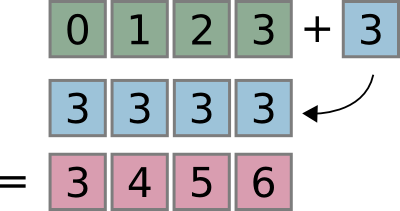
\includegraphics[height=0.7in, interpolate=true]{data/broadcast_scalar}
  \end{columns}
  \begin{itemize}
    \item Allows functions to take inputs that are not of the same shape
    \item 2 rules -
      \begin{enumerate}
      \item 1 is (repeatedly) prepended to shapes of smaller arrays
      \item Size 1 in a dimension changed to Largest size in that dimension
      \end{enumerate}
  \end{itemize}
\end{frame}

\begin{frame}[fragile]
  \frametitle{Broadcasting in 3D}
    \begin{lstlisting}
      >>> x = np.ones((3, 5))
      >>> y = np.ones(8)
      >>> (x[..., None] + y).shape
      (3, 5, 8)
    \end{lstlisting}
    \begin{figure}
      \begin{center}
      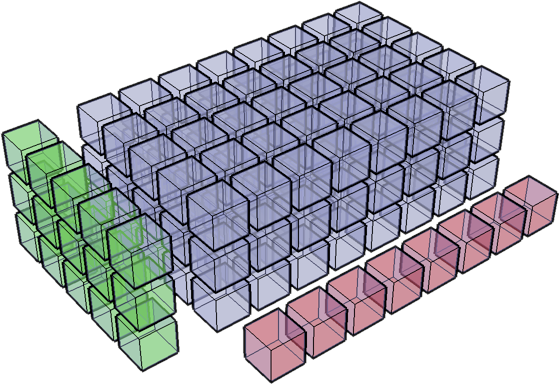
\includegraphics[height=1.5in, interpolate=true]{data/array_3x5x8}        
      \end{center}
    \end{figure}
\end{frame}

\begin{frame}[fragile]
  \frametitle{Copies \& Views}
  Try it!
  \vspace{-0.1in}
  \begin{lstlisting}
    >>> a = np.arange(1,9); a.shape=3,3
    >>> b = a
    >>> b is a
    >>> b[0,0]=0; print a
    >>> c = a.view()
    >>> c is a
    >>> c.base is a
    >>> c.flags.owndata
    >>> d = a.copy()
    >>> d.base is a
    >>> d.flags.owndata
  \end{lstlisting}
\end{frame}

\begin{frame}[fragile]
  \frametitle{Copies \& Views}
  Try it!
  \vspace{-0.1in}
  \begin{lstlisting}
    >>> b = a[0,1:3]
    >>> c = a[0::2,0::2]
    >>> a.flags.owndata
    >>> b.flags.owndata
    >>> b.base
    >>> c.base is a
  \end{lstlisting}
  \begin{itemize}
  \item Slicing and Striding just reference the same memory
  \item They produce views of the data, not copies
  \end{itemize}
\end{frame}

\begin{frame}[fragile]
  \frametitle{Copies contd \ldots}
  \begin{lstlisting}
    >>> b = a[np.array([0,1,2])]
    array([[1, 2, 3],
           [4, 5, 6],
           [7, 8, 9]])
    >>> b.flags.owndata
    >>> abool=np.greater(a,2)
    >>> c = a[abool]
    >>> c.flags.owndata
  \end{lstlisting}
  \begin{itemize}
  \item Indexing arrays or Boolean arrays produce copies
  \end{itemize}
\inctime{15}
\end{frame}

\section{SciPy}
\subsection{Introduction}
\begin{frame}
    {Intro to SciPy}
  \begin{itemize}
  \item \url{http://www.scipy.org}
  \item Open source scientific libraries for Python
  \item Based on NumPy
    \end{itemize}
\end{frame}

\begin{frame}
  \frametitle{SciPy}
  \begin{itemize}
  \item Provides:
    \begin{itemize}
    \item Linear algebra
    \item Numerical integration
    \item Fourier transforms
    \item Signal processing
    \item Special functions
    \item Statistics
    \item Optimization
    \item Image processing
    \item ODE solvers
    \end{itemize}
  \item Uses LAPACK, QUADPACK, ODEPACK, FFTPACK etc. from netlib
  \end{itemize}
\end{frame}

\begin{frame}[fragile]
  \frametitle{SciPy - Functions \& Submodules}
  \begin{itemize}
    \item All \typ{numpy} functions are in \typ{scipy} namespace
    \item Domain specific functions organized into subpackages
    \item Subpackages need to be imported separately
  \end{itemize}
  \begin{lstlisting}
    >>> from scipy import linalg
  \end{lstlisting}
\end{frame}

\subsection{Linear Algebra}
\begin{frame}[fragile]
  \frametitle{Linear Algebra}
  Try it!
  \begin{lstlisting}
    >>> import scipy as sp
    >>> from scipy import linalg
    >>> A=sp.mat(np.arange(1,10))
    >>> A.shape=3,3
    >>> linalg.inv(A)
    >>> linalg.det(A)
    >>> linalg.norm(A)
    >>> linalg.expm(A) #logm
    >>> linalg.sinm(A) #cosm, tanm, ...
  \end{lstlisting}
\end{frame}

\begin{frame}[fragile]
  \frametitle{Linear Algebra ...}
  Try it!
  \begin{lstlisting}
    >>> A = sp.mat(np.arange(1,10))
    >>> A.shape=3,3
    >>> linalg.lu(A)
    >>> linalg.eig(A)
    >>> linalg.eigvals(A)
  \end{lstlisting}
\end{frame}

\begin{frame}[fragile]
  \frametitle{Solving Linear Equations}
  \begin{align*}
    3x + 2y - z  & = 1 \\
    2x - 2y + 4z  & = -2 \\
    -x + \frac{1}{2}y -z & = 0
  \end{align*}
  To Solve this, 
  \begin{lstlisting}
    >>> A = sp.mat([[3,2,-1],[2,-2,4]
                  ,[-1,1/2,-1]])
    >>> B = sp.mat([[1],[-2],[0]])
    >>> linalg.solve(A,B)
  \end{lstlisting}
\inctime{15}
\end{frame}

\subsection{Integration}
\begin{frame}[fragile]
  \frametitle{Integrate}
  \begin{itemize}
    \item Integrating Functions given function object
    \item Integrating Functions given fixed samples
    \item Numerical integrators of ODE systems
  \end{itemize}
  Calculate the area under $(sin(x) + x^2)$ in the range $(0,1)$
  \begin{lstlisting}
    >>> def f(x):
            return np.sin(x)+x**2
    >>> integrate.quad(f, 0, 1)
  \end{lstlisting}
\end{frame}

\begin{frame}[fragile]
  \frametitle{Integrate \ldots}
  Numerically solve ODEs\\
  \begin{align*}
  \frac{dx}{dt}&=-e^{-t}x^2\\ 
           x&=2 \quad at \ t=0
  \end{align*}
  \begin{lstlisting}
>>> def dx_dt(x,t):
        return -np.exp(-t)*x**2
>>> t=np.linspace(0,2,100)
>>> x=integrate.odeint(dx_dt, 2, t)
>>> plt.plot(x,t)
  \end{lstlisting}
\inctime{10}
\end{frame}

\subsection{Interpolation}
\begin{frame}[fragile]
  \frametitle{Interpolation}
  Try it!
  \begin{lstlisting}
>>> from scipy import interpolate
>>> interpolate.interp1d?
>>> x = np.arange(0,2*np.pi,np.pi/4)
>>> y = np.sin(x)
>>> fl = interpolate.interp1d(
            x,y,kind='linear')
>>> fc = interpolate.interp1d(
             x,y,kind='cubic')
>>> fl(np.pi/3)
>>> fc(np.pi/3)
  \end{lstlisting}
\end{frame}

\begin{frame}[fragile]
  \frametitle{Interpolation - Splines}
  Plot the Cubic Spline of $sin(x)$
  \begin{lstlisting}
>>> tck = interpolate.splrep(x,y)
>>> X = np.arange(0,2*np.pi,np.pi/50)
>>> Y = interpolate.splev(X,tck,der=0)
>>> plt.plot(x,y,'o',x,y,X,Y)
>>> plt.show()
  \end{lstlisting}
\inctime{10}
\end{frame}

\subsection{Signal Processing}
\begin{frame}[fragile]
  \frametitle{Signal \& Image Processing}
    \begin{itemize}
     \item Convolution
     \item B-splines
     \item Filtering
     \item Filter design
     \item IIR filter design
     \item Linear Systems
     \item LTI Reresentations
     \item Waveforms
     \item Window functions
     \item Wavelets
    \end{itemize}
\end{frame}

\begin{frame}[fragile]
  \frametitle{Signal \& Image Processing}
  Applying a simple median filter
  \begin{lstlisting}
>>> from scipy import signal, ndimage
>>> from scipy import lena
>>> A=lena().astype('float32')
>>> B=signal.medfilt2d(A)
>>> imshow(B)
  \end{lstlisting}
  Zooming an array - uses spline interpolation
  \begin{lstlisting}
>>> b=ndimage.zoom(A,0.5)
>>> imshow(b)
  \end{lstlisting}
    \inctime{5}
\end{frame}

\begin{frame}[fragile]
  \frametitle{Problems}
  The Van der Pol oscillator is a type of nonconservative oscillator with nonlinear damping. It evolves in time according to the second order differential equation:
  \begin{equation*}
  \frac{d^2x}{dt^2}+\mu(x^2-1)\frac{dx}{dt}+x= 0
  \end{equation*}
  Make a plot of $\frac{dx}{dt}$ vs. $x$.
\inctime{30}
\end{frame}
\begin{frame}{Summary}
  \begin{itemize}
    \item Advanced NumPy
    \item SciPy
      \begin{itemize}
        \item Linear Algebra
        \item Integration
        \item Interpolation
        \item Signal and Image processing
      \end{itemize}
  \end{itemize}
\end{frame}
\end{document}

- Numpy arrays (30 mins)
    - Matrices
    - random number generation.
    - Image manipulation: jigsaw puzzle.
    - Monte-carlo integration.
